\chapter{Útkereső algoritmus}

A hexagonok és a négyzetek esetén az útkeresés csak egy ponton különbözik (szomszédok száma) ezért az egyszerűség kedvéért csak a négyzethálónál mutatom be.

\section{Algoritmusok}

A kereső algoritmusokat két pont közötti út megtalálására alkalmazzuk. 
A kereső algoritmusoknak több fajtája van, ezek különbözőképpen közelítik meg a problémát. 
\newline
\newline Az egyik csoport minden esetben talál egy megoldást ami nem feltétlenül a legrövidebb út viszont egy elfogadható közelítése annak (\textit{A algoritmusok}). Ezek az algoritmusok széleskörűen alkalmazhatóak ellentétben a másik csoporttal, mivel azok csak speciális esetekben használhatóak, mivel ezekhez további információk szükségesek a gráfról, amik nem minden esetben állnak rendelkezésünkre.
\newline A másik csoport ami minden esetben az optimális útvonalat találja meg, ha az létezik (\textit{A* algoritmus}).
\newline
\newline Az általános algoritmusok úgy keresik a megoldást, hogy a kezdő ponttól kiindulva végignézik a szomszédos csomópontokat és ezt ismétlik mindaddig amíg meg nem találják a végpontot. Az általános algoritmusok mint például a \textit{szélességi keresés} algoritmus is megtalálja az útvonalat ha megadjuk az ehhez szükséges időt, viszont olyan megoldások amik ''ismerik'' a gráfot általánosságban hamarabb elérik a célt. Gondoljuk csak végig mennyivel egyszerűbb megtalálni egy tárgyat ha tudjuk milyen irányban keressük ellentétben azzal, hogyha minden irányban kellene keresnünk azt.
\newline
\newline Két problémát kell megoldanunk az útkereséssel kapcsolatban 
\begin{itemize}
\item első az útvonal megtalálása két pont között, 
\item a második az, hogy a legrövidebb utat találjuk meg. 
\end{itemize}

\noindent Olyan alapvető algoritmusok mint a \textit{szélességi
keresés} vagy a \textit{mélységben először keresés} nagyon egyszerűen megoldják az első problémánkat azáltal, hogy az összes lehetséges útvonalat bejárják. Ezek az algoritmusok $\mathcal{O}(|V| + |E|)$ (lineáris) futásidejűek, ahol $V$ a csúcsok száma és $E$ az élek száma.
\newline
\newline A legrövidebb út megtalálása már ennél jóval komplexebb probléma. 
\newline
\newline Edsger Dijkstra találta meg erre a problémára a megoldást 1956-ban. Az algoritmusából manapság már több változat is létezik. Dijkstra eredeti algoritmusa megtalálta a legrövidebb utat két csúcs között egy súlyozott gráfon, de manapság a leggyakoribb változata úgy változtatja meg az algoritmust, hogy egy megadott csúcsponthoz viszonyítva kiszámítja az összes többi csúcsponthoz vezető legrövidebb utat, ezáltal előállítva a legrövidebb út fát. Ennek a futásideje $\mathcal{O}(|E| + |V| log|V|)$. 
\newline
\newline A \textit{Bellman-Ford} algoritmus ugyanazt a problémát oldja meg mint a \textit{Dijkstra} algoritmus, viszont ez egy sokoldalúbb algoritmus, mivel az élek értéke negatív értéket is felvehet. Mindössze azt kell kizárni, hogy a gráf negatív összköltségű kört tartalmazzon. Negatív költségű él például úgy keletkezhet, hogy nagyobb bevételhez jutunk azon a szakaszon mint amennyi ráfordítással jár. A legrosszabb esetű futásideje $\mathcal{O}(|V||E|)$ (négyzetes idő), de bizonyos esetekben akár $\mathcal{O}(|V|)$ is lehet, ami azt jelenti, hogy legrosszabb esetben lassabb mint a \textit{Dijkstra}-féle algoritmus de akár gyorsabb is lehet. 
\newline
\newline Azonban nem szükséges az összes lehetséges útvonalat bejárni ahhoz, hogy megtaláljuk az optimális útvonalat. Olyan algoritmusok mint a \textit{Dijkstra} vagy az \textit{A*} stratégiája az, hogy heurisztikák segítségével eliminálja az olyan útvonalakat amik nem lehetségesek vagy nem vezetnek a megoldás felé. Ezáltal lehetővé téve, hogy elérjék az $\mathcal{O}(|E| log(|V|))$ futásidőt. 
\newline
\newline A fent említett algoritmusok a legjobb általános algoritmusok közé tartoznak amikkel előfeldolgozás nélkül is kilehet értékelni egy gráfot. Gyakorlatban elérhető még ezeknél is jobb idő komplexitású algoritmus, ha előfeldolgozzuk a gráfot.
\newline
\newline A leggyakrabban alkalmazott algoritmusok ismertetése:

\subsection{A szélességi keresés algoritmusa (breadth-first search)}
A \textit{szélességi keresés} egy egyszerűnek számító keresési algoritmus. A térképen minden egyes irányban egységes mértékben keres. Ez egy teljes keresés, ezáltal minden esetben a legrövidebb utat fogja megtalálni a célhoz. A keresés a gyökér csomóponttól indul és úgy folytatódik, hogy az összes csomópontot ami a gyökér csomópontból elérhető kiértékeli. Ezután ezekből a csomópontokból elérhető csomópontokat értékeli ki az algoritmus. Ez az algoritmus mindig egy adott mélységen lévő csomópontokat értékeli ki egyszerre és ezután halad tovább a következő szintre. Könnyen belátható, hogy az algoritmus a FIFO (first-in-first-out) elv alapján működik. Tehát azokat az elemeket értékeli ki először egy adott listáról amik először felkerültek a listára. Ezáltal belátható, hogy ez az algoritmus a legmagasabb szinten található cél csomópontot fogja megtalálni először. 

\begin{figure}[h!]
\centering
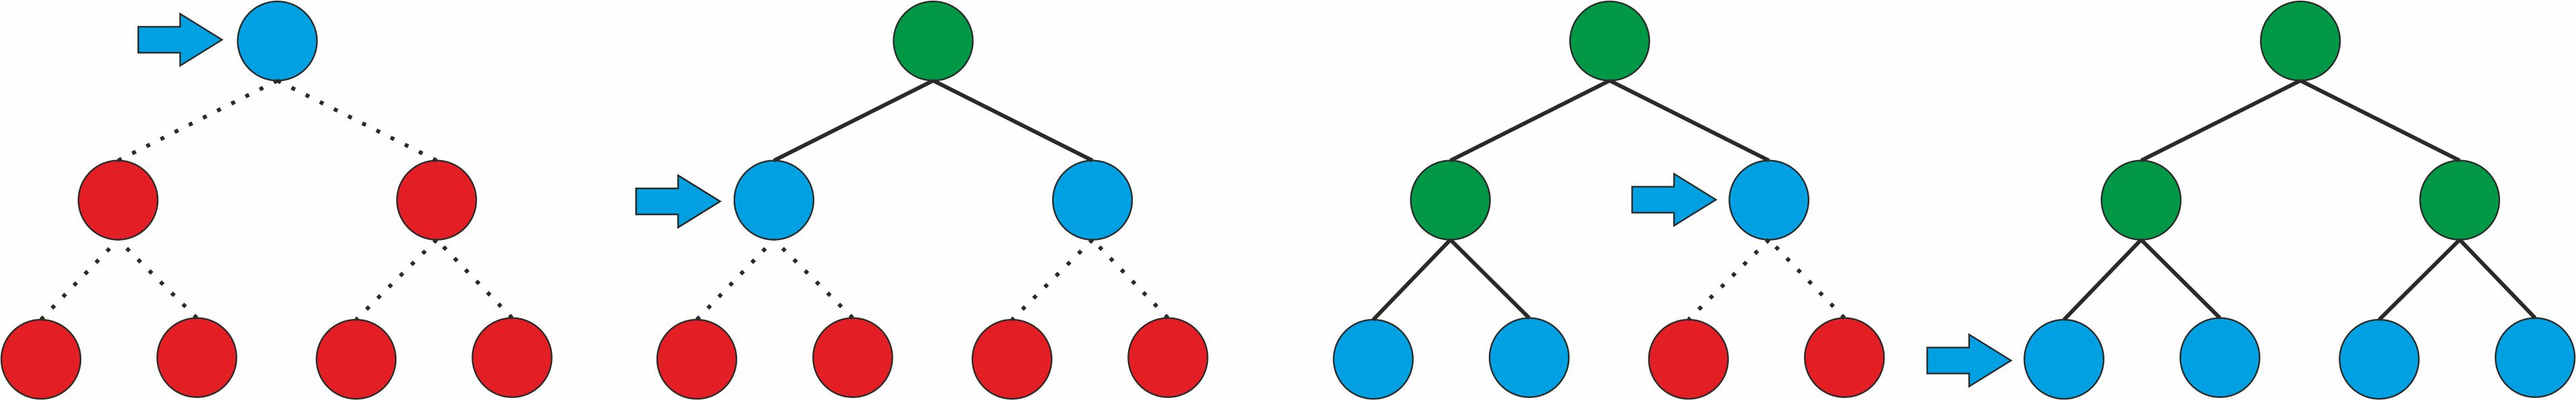
\includegraphics[scale=0.4]{kepek/breadth-first_search.jpg}
\caption{Szélességi keresés algoritmus lépései}
\label{fig:breadth-first_search}
\end{figure}

\noindent Mindazonáltal mivel ez egy teljes keresés az egész gráf kiértékelésre kerül, mivel nem feltétlenül a legmagasabban található cél csomóponthoz vezető úton jutunk el a leggyorsabban a célhoz, abban az esetben ha az éleknek különbözik a súlya. Ezért érdemes olyan esetekben használni amikor a gráf éleinek nincs súlya vagy egységes súlya van, mert abban az esetben elégséges lehet a legmagasabban található cél csomópontig eljutni.  Érdemes továbbá tisztázni, hogy ha a térképen egy darab célpontunk van az a gráfban több célcsomópontként is megjelenhet, mivel a gráf különböző útvonalai a különböző útvonalakat jelölik ugyanazon célhoz, de egyszerre akár több célunk is lehet a térképen.
\newline
\newline A szélességi keresés algoritmus legnagyobb hátránya a tárigénye. Vegyünk például egy hipotetikus állapotteret, ahol minden kifejtéskor $x$ darab új csomópontot kapunk állapotunk van. Tehát a gyökér kifejtésekor $x$ darab elemünk lesz. Második szinten $x^2$. Tegyük fel, hogy a cél csomópontunk n mélységben található, ekkor legrosszabb esetben $x^n - x$ csomópontot kell kiértékelnünk, mivel az utolsó mélységet már nem szükséges kiértékelnünk. 
\newline
\newline A szélességi keresés algoritmus egy nem informált keresés mivel a cél csomópontról nem rendelkezik információval. A továbbiakban csak informált keresésekről esik majd szó.

\subsection{Dijkstra algoritmus}

\noindent Gyakori példa a gráf alapú útkereső algoritmusra a \textit{Dijkstra} algoritmus. A szélességi keresés módszerrel ellentétben nem egységesen fedezi fel az utakat, hanem a kisebb útköltségűeket priorizálja. Ennek az algoritmusnak az elején szükségünk lesz egy kezdő csomópontra és egy listára a “Nyitott” csomópontoknak, ide kerülnek azok a csomópontok amiket még ki kell értékelnünk. Minden iterációban az a csomópont kerül kiértékelésre amelyiknek a legkisebb az útköltsége a kezdő csomóponttól mérve. Az útköltség függhet attól, hogy milyen területen haladunk (magassági viszonyok változásától, a talaj anyagától, időjárási viszonyoktól, egyéb környezeti viszonyoktól, ha az úton ellenség van akkor is megnövelhetjük az út költségét). Az algoritmus alapvetően súlyozott élek esetén működik, de használható súlyozatlan élek esetén is, ekkor a súlyozatlan élek értékét válasszuk 1-nek. Akkor kerül egy csomópont “lezárásra”, hogyha már az összes szomszédja hozzá lett adva a nyitott csomópontok listájához vagy már lezárásra került. Ez a folyamat addig ismétlődik amíg az algoritmus megtalálja az első útvonalat a célhoz (ami lehet akár az összes csomópont is). Mivel mindig a legkisebb útköltségre lévő út fog kiértékelődni, ezért amit először megtalál, az lesz a legrövidebb út. Tehát változatos útköltségek esetén érdemesebb a \textit{Dijkstra} algoritmust használni a szélességi keresés módszer helyett.

\subsection{A* algoritmus}

\noindent Az \textit{A*} algoritmus a \textit{Dijkstra} algoritmus tovább gondolása, amit gyorsasága és a pontossága miatt előszeretettel alkalmaznak játékok készítésekor, olyan esetekben, amikor csak egy konkrét végponthoz kell eljutni. A két algoritmus közötti fő különbség abban rejlik, hogy melyik csomópontot választja ki az algoritmus kiértékelésre a nyitott csomópontok közül. Ahhoz, hogy megértsük az \textit{A*} kiválasztási módszerét először meg kell ismernünk 3 fogalmat.

\begin{itemize}
\item \textit{G költség}: Az adott csomóponthoz vezető út költsége a kezdő csomóponthoz képest.
\item \textit{H költség (heurisztikus költség)}: A becsült távolság a célhoz képest.
\item \textit{F költség}: $F = G + H$. Ez az érték alapján kerül kiválasztásra a kiértékelendő csomópont.
\end{itemize}

\noindent A \textit{Dijkstra} algoritmussal ellentétben nem az útköltségek alapján priorizál hanem a célponttól lévő távolság alapján.
\newline
\newline A \textit{G költség} tulajdonképpen a \textit{Dijkstra} algoritmus használata és ezt egészíti ki az \textit{A*} algoritmus egy heurisztikus költséggel, ami azért szükséges, hogy kizárjuk a hosszabb útvonalakat. Heurisztikaként leggyakrabban a Manhattan-formulát szokták használni. Ha a heurisztikus költséget 0-ra ''állítjuk be'', akkor az algoritmus megegyezik a \textit{Dijkstra} algoritmussal.
\newline
\newline Az útkereső algoritmus készítéséhez szükséges ismernünk azt, hogy a térkép egy mezőjéről hogyan érhetőek el a szomszédos mezők és szükséges ismernünk a távolság számító algoritmusokat is. Mivel a távolság számító algoritmusokat már ismertettem korábban ezért most nézzük meg a szomszédokat.

\section{Szomszédok}

Ahhoz, hogy útkereső algoritmust tudjunk készíteni ismernünk kell, hogy a különböző alakzatok és koordináta-rendszerek esetén milyen algoritmussal érhetjük el az adott alakzat szomszédait. 
\newline
\newline Az algoritmusokat ebben a formában fogom megadni: $A \rightarrow B1, B2, B3 …$
(Az $''A''$ és $''B''$ pontokat $''u''$, $''v''$ koordináták segítségével fogom megadni.)

\subsection{Négyzet}
A négyzet esetén egyszerű dolgunk van, mert csak egyfajta koordináta-rendszerünk van.

$$
(u,v) \rightarrow (u,v+1) (u+1,v) (u,v-1), (u-1,v)
$$

\subsection{Hexagon}

Hexagon esetén több fajta koordináta-rendszerünk is lehet.

\subsubsection{Kocka koordináta-rendszer (Cube coordinates)}

\noindent Ahhoz, hogy elmozduljunk eggyel meg kell változtatnunk egyet a három kocka koordináta közül $+1$-el és egy másikat $-1$-el (a változtatások összege $0$ kell, hogy legyen). Három koordinátát lehet megváltoztatni $+1$-el, a másik két lehetséges koordináta közül az egyiket kell csökkenteni $-1$-el. Ez hat lehetséges változatot eredményez. Mindegyik megfeleltethető a hexagon egyik irányának. A lehető legegyszerűbb és leggyorsabb megoldás az, ha az összes lehetséges permutációt előre kikalkuláljuk és beleírjuk egy táblázatba ( Cube($dx, dy, dz$)).
\newline
\newline Algoritmus: 
\begin{cpp}
Cube[] cubeDirections = 
{ 
   Cube(+1, -1,  0), Cube(+1,  0, -1), Cube( 0, +1, -1),
   Cube(-1, +1,  0), Cube(-1,  0, +1), Cube( 0, -1, +1) 
};

public Cube CubeDirection(int direction)
{
   return cubeDirections[direction];
}

public Cube CubeNeighbor(Cube cube, int direction)
{
   return Cube
   (
      cube.x + cubeDirections[direction].x, 
      cube.y + cubeDirections[direction].y, 
      cube.z + cubeDirections[direction].z
   );
}
\end{cpp}

\subsubsection{Tengely koordináta-rendszer (Axial coordinates)}

\noindent A kocka koordináta-rendszer veszük alapul. Mégpedig úgy, hogy a Cube($ dx, dy, dz$) koordinátákat átalakítjuk Axial($ dx, dz$) -re.
\newline
\newline Algoritmus:
\begin{cpp}
Axial[] axialDirections = 
{ 
   Axial(+1,  0), Axial(+1, -1), Axial( 0, -1),
   Axial(-1,  0), Axial(-1, +1), Axial( 0, +1)
};

public Axial AxialDirection(int direction)
{
   return axialDirections[direction];
}

public Axial AxialNeighbor(Axial axial, int direction)
{
   return Axial
   (
      axial.x + axialDirections[direction].x, 
      axial.y + axialDirections[direction].y, 
   );
}
\end{cpp}

\subsubsection{Eltolásos koordináta-rendszer (Offset coordinates)}

\noindent Eltolásos koordináta-rendszer esetén a lépések változnak annak a függvényében, hogy hol állunk a hálóban. Ha mi egy eltolt oszlopban/sorban állunk akkor a szabály eltér attól mintha egy nem eltolt oszlopban/sorban állnánk.
\newline
\newline Ahogy a korábbi esetekben úgy most is kell készítenünk egy táblázatot amiben azt tároljuk majd, hogy a különböző tengelyeken mennyit kell hozzáadni, hogy elérjük a szomszédokat. De ebben az esetben most két tömbre lesz szükségünk, az egyik a páros sor/oszlop a másik pedig a páratlan sor/oszlop esetére.
\newline
\newline A táblázat különbözik mind a négy eltolásos módszernél.
\newline
\newline Páratlan sor: 
\begin{cpp}
OddRow[,] oddRowDirections = 
{ 
   [ 
      OddRow(+1,  0), OddRow( 0, -1), OddRow(-1, -1),
      OddRow(-1,  0), OddRow(-1, +1), OddRow( 0, +1) 
   ],
   [ 
      OddRow(+1,  0), OddRow(+1, -1), OddRow( 0, -1),
      OddRow(-1,  0), OddRow( 0, +1), OddRow(+1, +1) 
   ]
};

public OddRow OddRowNeighbor(OddRow oddRow, int direction)
{
   int parity = oddRow.row \% 2;
   OddRow dir = oddRowDirections[parity][direction];
   return OddRow(oddRow.col + dir.col, oddRow.row + dir.row);
}   
\end{cpp}

Páros sor: 
\begin{cpp}  
EvenRow[,] evenRowDirections = 
{ 
   [
      EvenRow(+1,  0), EvenRow(+1, -1), EvenRow( 0, -1),
      EvenRow(-1,  0), EvenRow( 0, +1), EvenRow(+1, +1) 
   ],
   [ 
      EvenRow(+1,  0), EvenRow( 0, -1), EvenRow(-1, -1),
      EvenRow(-1,  0), EvenRow(-1, +1), EvenRow( 0, +1) 
   ]
};

public EvenRow EvenRowNeighbor(EvenRow evenRow, int direction)
{
   int parity = evenRow.row \% 2;
   EvenRow dir = evenRowDirections[parity][direction];
   return EvenRow(evenRow.col + dir.col, evenRow.row + dir.row);
}   
\end{cpp}

Páratlan oszlop: 
\begin{cpp}
OddColumn[,] oddColumnDirections = 
{ 
   [ 
      OddColumn(+1,  0), OddColumn(+1, -1), OddColumn( 0, -1),
      OddColumn(-1, -1), OddColumn(-1,  0), OddColumn( 0, +1) 
   ],
   [ 
      OddColumn(+1, +1), OddColumn(+1,  0), OddColumn( 0, -1),
      OddColumn(-1,  0), OddColumn(-1, +1), OddColumn( 0, +1) 
   ]
};

public OddColumn OddColumnNeighbor(OddColumn oddColumn, int direction)
{
   int parity = oddColumn.col \% 2;
   OddColumn dir = oddColumnDirections[parity][direction];
   return OddColumn(oddColumn.col + dir.col, oddColumn.row + dir.row);
}   
\end{cpp}

Páros oszlop: 
\begin{cpp}
EvenColumn[,] evenColumnnDirections = 
{ 
   [ 
      EvenColumn(+1, +1), EvenColumn(+1,  0), EvenColumn( 0, -1),
      EvenColumn(-1,  0), EvenColumn(-1, +1), EvenColumn( 0, +1) 
   ],
   [  
      EvenColumn(+1,  0), EvenColumn(+1, -1), EvenColumn( 0, -1),
      EvenColumn(-1, -1), EvenColumn(-1,  0), EvenColumn( 0, +1) 
   ]
};

public EvenColumn EvenColumnNeighbor
(
   EvenColumn evenColumn, 
   int direction
)
{
   int parity = evenColumn.col \% 2;
   EvenColumn dir = evenColumnDirections[parity][direction];
   return EvenColumn(evenColumn.col + dir.col, evenColumn.row + dir.row);
}   
\end{cpp}

\subsubsection{Átlós szomszédok}

\noindent Az “átlós” szomszédok a kocka koordináták esetén úgy működik, hogy a lehetséges három koordináta közül az egyiket $ \pm 2$ -vel, míg a másik kettőt $\mp 1$ -el módosítjuk, hogy a három koordináta összege mindig $0$ legyen.

\begin{figure}[h!]
\centering
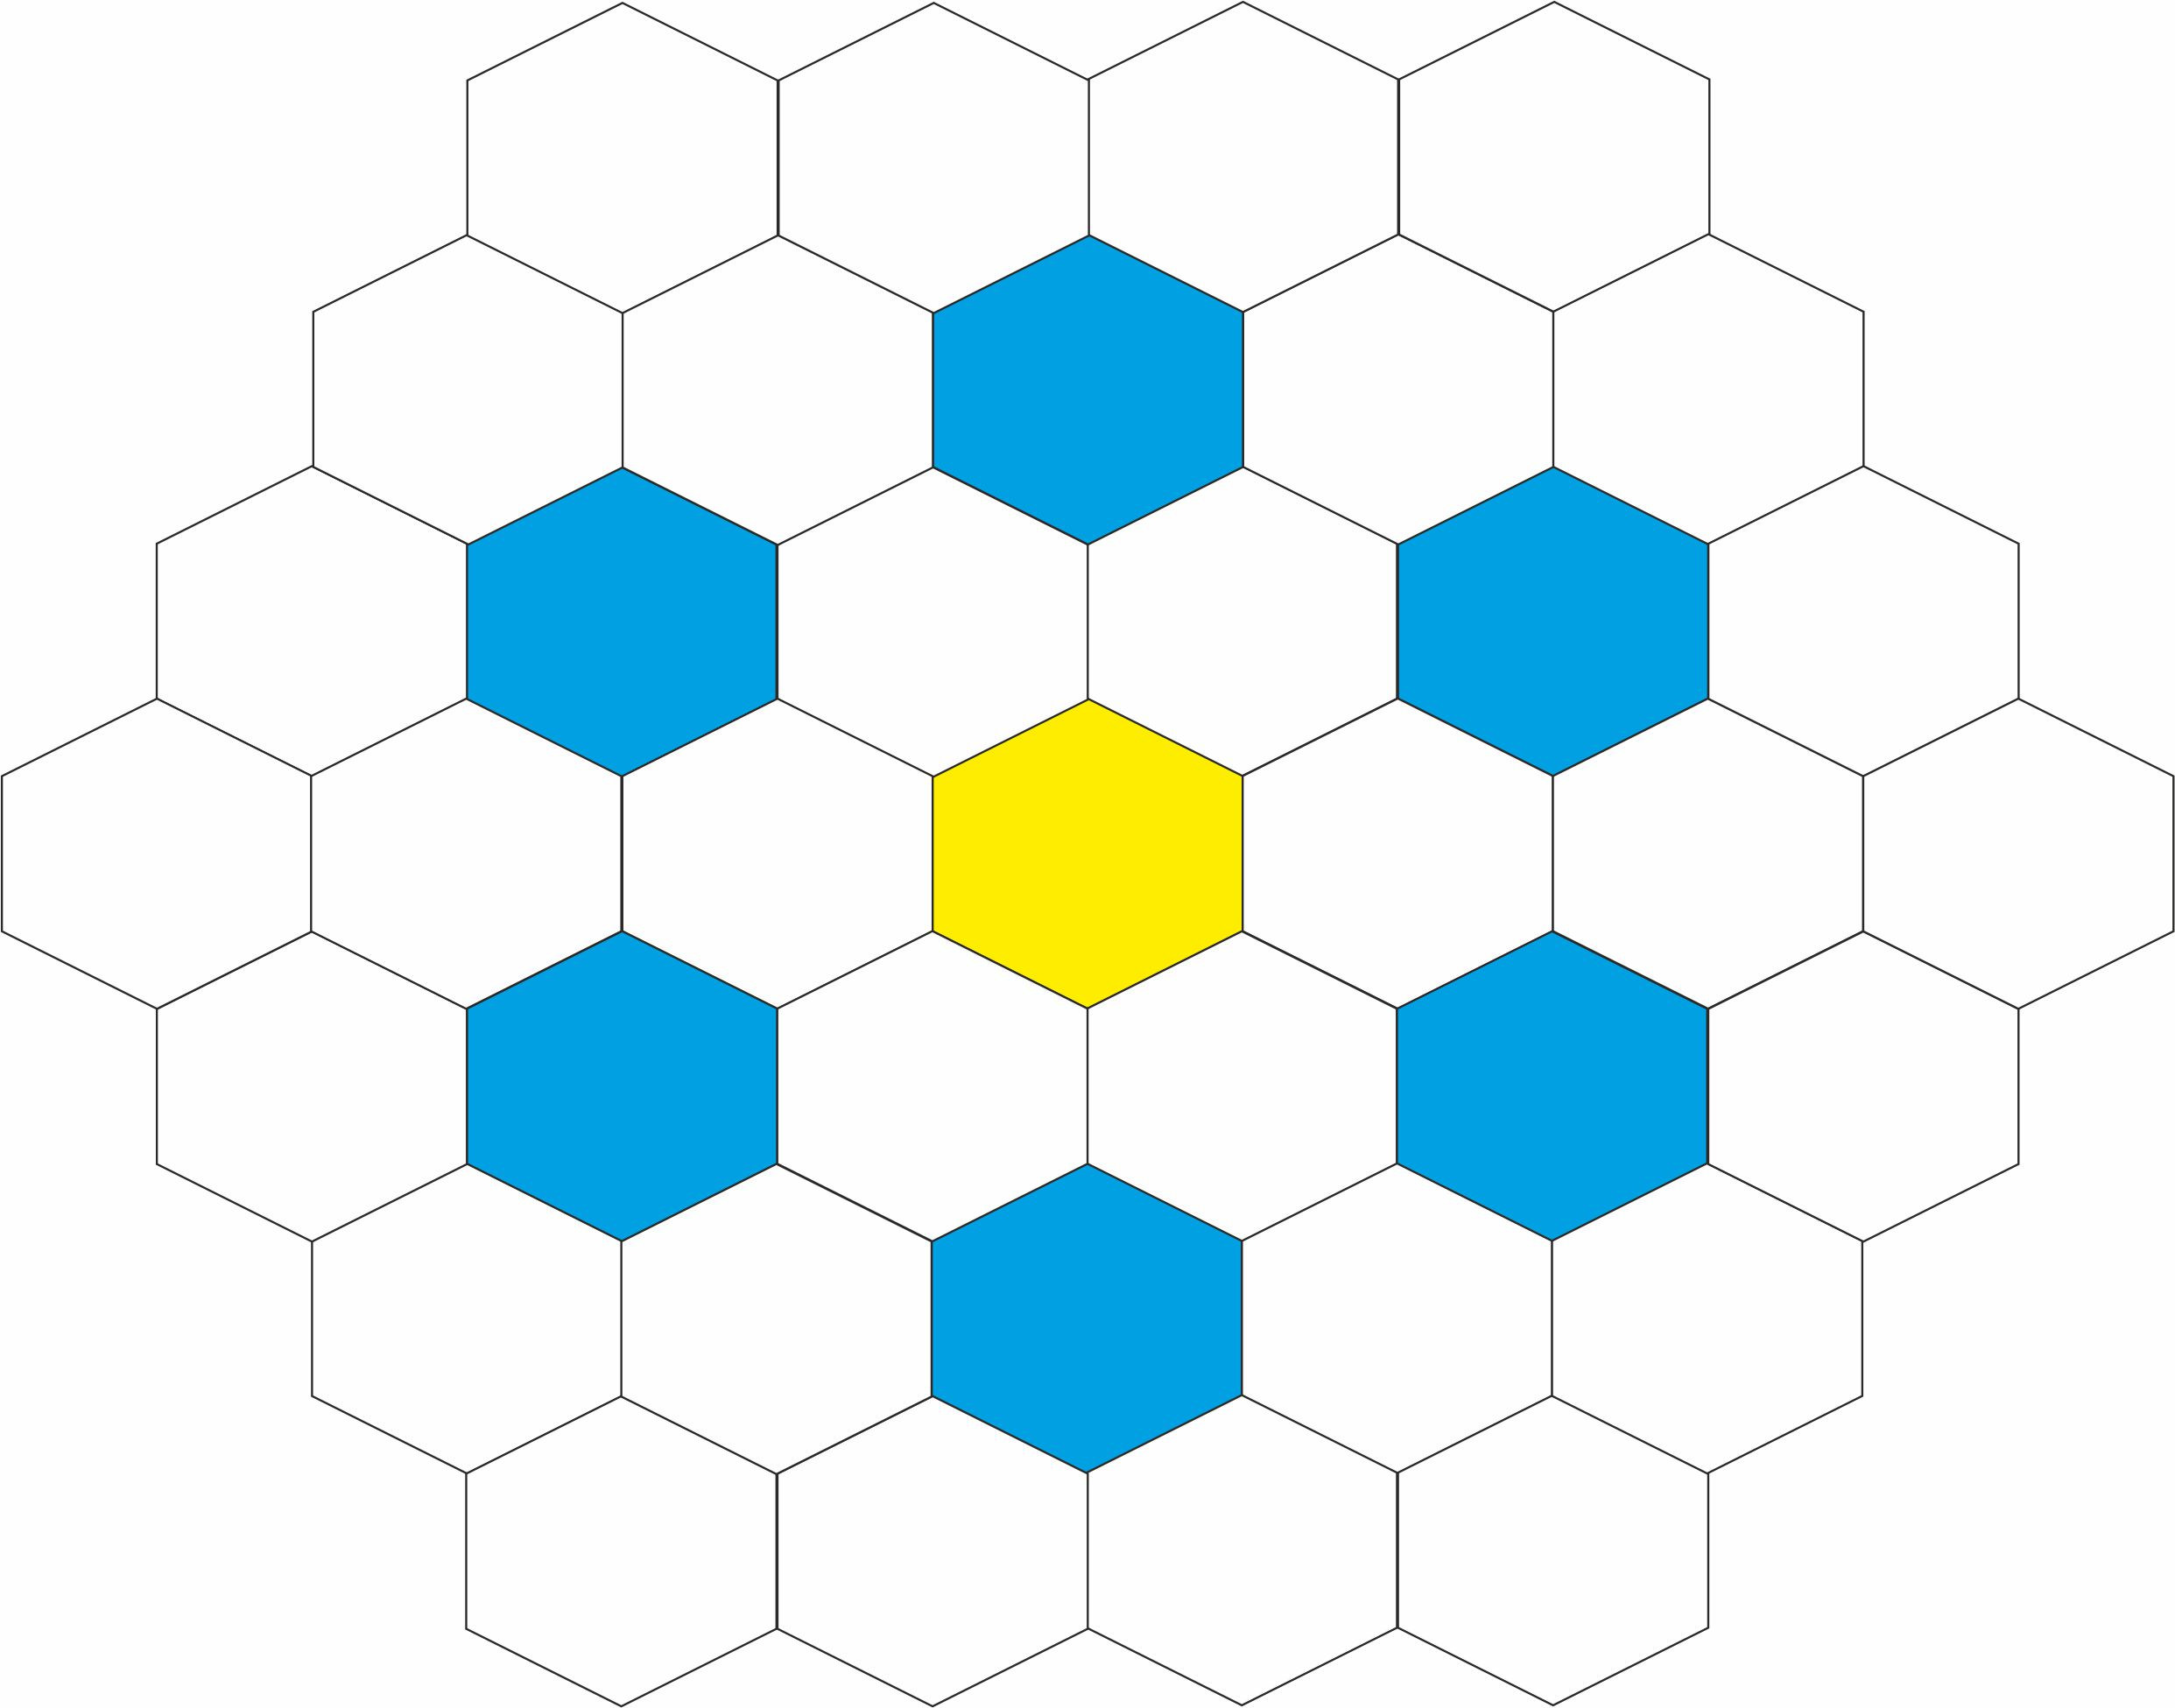
\includegraphics[scale=0.3]{kepek/Diagonals.jpg}
\caption{"Átlós" szomszédok hexagon háló esetén}
\label{fig:Diagonals}
\end{figure}

\noindent Algoritmus:
\begin{cpp}  
Diagonals[] diagonalsDirections = 
{ 
   Diagonals(+2, -1, -1), Diagonals(+1, +1, -2), Diagonals(-1, +2, -1), 
   Diagonals(-2, +1, +1), Diagonals(-1, -1, +2), Diagonals(+1, -2, +1)
};

public Diagonals DiagonalsNeighbor(Diagonals diagonals, int direction)
{
   return Diagonals
   (
      diagonals.x + diagonalsDirections[direction].x, 
      diagonals.y + diagonalsDirections[direction].y, 
      diagonals.z + diagonalsDirections[direction].z
   );
}         
\end{cpp}

\noindent Tengelyes koordináta-rendszer használata esetén is lehetséges az algoritmus használata.